\section{Multi-Agent Reinforcement Learning}
I will now turn to examine the generalization of single-agent MDPs to settings that involve multiple agents
and the dynamics between them. Although the field of multi-agent reinforcement learning spans many possible
approaches, the unifying framework underlying all of them is that of a Stochastic Game which bares its roots in 
Game Theory. Within the scope of this project, a particularly recent advancement at the intersection of
reinforcement learning and games with an infinite number of players, newly developed mean field multi agent
learning algorithms are also discussed.
\subsection{Stochastic Games}
Many of the concepts introduced within the framework of a markov decision process have their
origins in decision theory, particularly expected utility theory \cite{sutton2018reinforcement}.
As such many of the concepts introduced so far have synonymous terminology in game theory, which
I will introduce and make use of for the convenience of describing later topics. \\

A normal form game is defined by a set of players (agents) who take actions within an environment
that maximise their expected discounted payoffs $\mathbb{E}[\gamma G_{t+1}]$ according to some strategy
$\pi$. Normal form games are defined to be \textbf{non-cooperative}, \textbf{static} and of \textbf{complete information},
indicating that although agent's priorities may align, they each are self interested with respect
to their own reward function. Static defines the property that each player chooses their action 
without knowledge of the actions being played by other players at the current time-step. Complete knowledge
is defined not only in terms of complete knowledge of the environment, but also the knowledge that
every agent knows that every agent knows that every other agent has knowledge of the environment,\emph{ad infimum}. \\

A stochastic game is a generalization over both MDPs and repeated games (games played over a span of time)
which can be described as a collection of normal form games which are played by the agents where 
the game played at any point in time probabilistically depends on the previously game played
and the actions taken therein \cite{shoham2009multiagent}. 
Formally, a stochastic game is defined as the tuple $\Gamma \coloneqq (\mathcal{S}, \mathcal{A}^1, \hdots, \mathcal{A}^n, r^1, \hdots r^N, p, \gamma)$
where $\mathcal{S}$ denotes the familiar state space in which the agents act in,  $\mathcal{A}^j$ represents the action
space of agent $j \in {1, \hdots, N}$, the actions in turn are drawn from some stationary distribution $p = \mathcal{S} \times \mathcal{A}^1 \times \hdots \times \mathcal{A}^n \rightarrow \Omega(\mathcal{S})$
where $\Omega(\mathcal{S})$ represent the collection of distributions over the state space \cite{Yang2018}. 
The primary departure of interest from the previously introduced setting is the reward 
function $r^j$ of each agent as they now take into consideration the actions of all the other agents:
\begin{equation}
    r^j : \mathcal{S}\times \mathcal{A}^1\times \hdots \times \mathcal{A}^n \rightarrow \mathbb{R}
\end{equation}
Likewise, we also define the joint strategy of all agents:
\begin{equation}
    \boldsymbol \pi \triangleq [\pi^1, \pi^2, \hdots, \pi^N]
\end{equation}
From this we can derive the Q and value function of such agents:
\begin{equation}
    \begin{gathered}
        v_{\boldsymbol \pi}^j(s) = v^j(s;\boldsymbol \pi ) = \sum_{t=0}^{\infty} \gamma^t \E_{\boldsymbol \pi, p}[r^j_t \mid s_0 = s, \boldsymbol \pi] \\
        Q_\pi^j(s, \mathbf{a}) = r^j(s, \mathbf{a}) + \gamma \E_{s' \backsim p}[v^j_{\boldsymbol \pi}(s')]
    \end{gathered}
\end{equation}
In multi-agent reinforcement learning, each agent aims to learn an optimal policy to maximize
its respective value function, indicating that any optimal value function must
take into account not only the agent's policy, but the joint policy of all other agents;
following the logic set out in equations (2.29-32):
\begin{equation}
    v^j(s; \boldsymbol \pi_*) = v^j(s;\pi^j_*,\boldsymbol \pi^{-j}_*) \geq v^j(s;\pi^j,\boldsymbol \pi^{-j}_*)
\end{equation}
Where $\mathbf{a} \triangleq [a^1, \hdots, a^N]$ is defined as the joint action over all agents.
Here the optimal joint policy $\boldsymbol \pi_*$ as been decomposed into the policy of the individual
agent $\pi^j$ and the joint policy of all other agents except j $\boldsymbol \pi_*^{-j}$.
In game theoretic terms, the optimal joint policy represents the \emph{Nash equilibrium} of the
sytem, defined as the deterministic joint optimal strategy from which the agents do not deviate from
because it maximises the expected discounted payoff for all agents.
In a nash equilibrium, each agent acts with the best response $\pi^j_*$ to other provided that
that all other agents adhere to $\boldsymbol \pi^{-j}_*$. \cite{Hu2003} defined an iterative 
procedure as follows:
\begin{itemize}
    \item Solve the Nash equilibrium of the current state game
    \item Bootstrap the current estimation of the Q value for each learning with the new Nash equilibrium value
\end{itemize}
The conjugation of these operations is collectively define the \emph{Nash operator} $\mathscr{H}^{Nash}$:
\begin{equation}
    \mathscr{H}^{Nash}Q(s, \mathbf{a}) = \E_{s' \backsim p}[\mathbf{r}(s, \mathbf{a}) + \gamma \mathbf{v}^{Nash}(s')]
\end{equation}
Where $\mathbf{v}$ defines the joint value function governing the value of states under the Nash equilibrium and $\mathbf{r}$
represents joint rewards of all agents.
\cite{Hu2003} show that this operator forms a contraction mapping in similar fashion to (2.61), indicating
that the Q function will eventually converge to the values that constitute the Nash equilibrium
of the game, the \emph{Nash Q value}. \\

One can see that the dimension of the cartesian product of the joint action $\mathbf{a}$ 
grows proportionally with respect to the number agents, this limitation was initially thought
to be computationally intractable for a large to infinte number of players, \cite{Yang2018}
circumvent this limitation by introducing the mean field game framework.
\subsection{Mean Field Games}
Owing it's origin to mean field theories in physics, mean field games
first pioneered by \cite{Lasry2007} examine classes of games that have extremely large
numbers of players,particularly in the infinite limit. Many of the intractabilities
associated with games of many players simplify in the infinite limit; instead of considering
the interaction of the agent with all other agents, we consider the pairwise interaction
between the agent and some virtual \emph{mean} agent. Under the standard
assumptions of mean-field approximation, each agent is assumed to be
\emph{indistinguishable} and \emph{interchangable}, indicating that given an indexed
set of agents, the ordering of their indices does not have an effect on their
interactions, this assumption will be relaxed later when multiple types of agents
are introduced. Within the context of reinforcement
learning, \cite{Yang2018} factorize the Q function into only the pairwise local interactions
in the \emph{neighbourhood} of the agent:
\begin{equation}
    \begin{gathered}
        Q^j = \frac{1}{N^j} \sum_{k \in \mathcal{N}(j)}Q^j(s,a^j, a^k) \\
        N^j = \vert \mathcal{N}(j) \vert
    \end{gathered}
\end{equation}
Where $\mathcal{N}(j)$ is the index set of neighbouring agents determined by different applications
and $a^j$ is the discrete acion space of agent $j$ and $a^k$ represents the \emph{empirical distribution}
of the one-hot encoded neighbouring agent's actions:
\begin{equation}
    \begin{gathered}
        a^1 = \begin{bmatrix}
            1\\0\\0\\\vdots\\0
        \end{bmatrix}_1
        \;a^2 = \begin{bmatrix}
            0\\1\\0\\\vdots\\0
        \end{bmatrix}_2 \; \hdots\:
        a^N = \begin{bmatrix}
            0\\0\\0\\\vdots\\1
        \end{bmatrix}_N\\
        \mathbf{a}^k \approx \mathbf{a}^{-j} \;\; \text{where} \;\; a^{-j} = \frac{1}{N^j} \sum_k a^k
    \end{gathered}
\end{equation}
Although this reduces the complexity significantly, it still preserves global interactions implicitly
\cite{Blume1993}. Assuming that the joint Q function is \emph{Lipschitz continuous}, \cite{Yang2018}
show that if we examine the interaction between a central agent $j$ and an arbitary neighbour $k$ as $Q^j(s,a^j,a^k)$
and evaluate the second order Taylor approximation of this interaction, we find that from
the perspective of agent $j$, it's immediate neighbour will choose it's actions based on its
own respective neighbours. This is tantamount to the action taken by immediate neighbour $k$ being determined
according to some external action \emph{distribution} of it's own neighbours, and so by the findings of \cite{Blume1993}
one can approximate the pairwise interactions of each neighbour as that between $j$
and the virtual mean agent $k$ that captures the mean effect of all of the neighbours within $j$'s neighbourhood
while conserverving global interactions implicitly.\\

This is depicted in figure (2.11) where the central agent $j$ is shown as the node in red, the central node
only considers the actions taken by its immediate neighbours on the lattice shown in in blue, rather than 
taking into considerations the actions of all nodes on the lattice.
\begin{figure}[!htb]
    \centering
        \caption{Mean field interactions}
        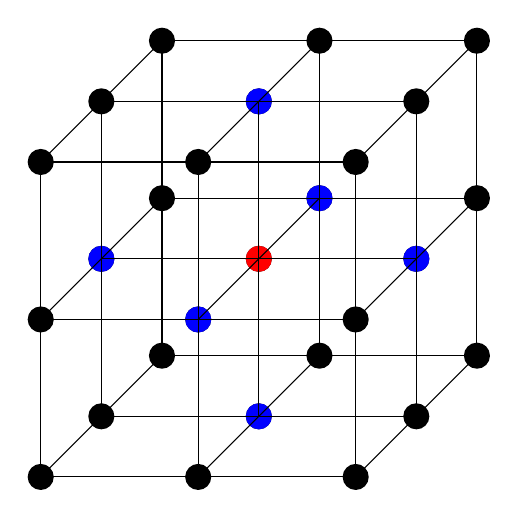
\begin{tikzpicture}

            \def \dx{2};
            \def \dy{2};
            \def \dz{2};
            \def \nbx{3};
            \def \nby{3};
            \def \nbz{3};
            
            \foreach \x in {1,...,\nbx} {
                \foreach \y in {1,...,\nby} {
                    \foreach \z in {1,...,\nbz} {
                        \node at (\x*\dx,\y*\dy,\z*\dz) [circle, fill=black] {};
                    }
                }
            }
            \node at (2*\dx,2*\dy,2*\dz) [circle, fill=red] {};
            \node at (2*\dx,3*\dy,2*\dz) [circle, fill=blue] {};
            \node at (2*\dx,1*\dy,2*\dz) [circle, fill=blue] {};
            \node at (1*\dx,2*\dy,2*\dz) [circle, fill=blue] {};
            \node at (3*\dx,2*\dy,2*\dz) [circle, fill=blue] {};
            \node at (2*\dx,2*\dy,1*\dz) [circle, fill=blue] {};
            \node at (2*\dx,2*\dy,3*\dz) [circle, fill=blue] {};
            % z lines
            \foreach \x in {1,...,\nbx} {
                \foreach \z in {1,...,\nbz}{
                    \draw (\x*\dx,\dy,\z*\dz) -- ( \x*\dx,\nby*\dy,\z*\dz);
                }
            }
            
            % x lines
            \foreach \y in {1,...,\nbx} {
                \foreach \z in {1,...,\nbz}{
                    \draw (\dx,\y*\dy,\z*\dz) -- ( \nbx*\dx,\y*\dy,\z*\dz);
                }
            }
            
            % y lines
            \foreach \x in {1,...,\nbx} {
                \foreach \y in {1,...,\nbz}{
                    \draw (\x*\dx,\y*\dy,\dz) -- ( \x*\dx,\y*\dy,\nbz*\dz);
                }
            }
            
            \end{tikzpicture}
\end{figure}
\cite{Yang2018} model the distribution over the actions of the virtual mean agent
with a \emph{Boltzmann policy} at time $t$ parameterised by the empirical distribution (2.73)
of the neighbouring actions:
\begin{equation}
    \pi^j_t(a^j \mid s, a^{-j}) =\frac{\exp(-\beta Q^j_t(s,a^j,a^{-j}))}{\sum_{a^j \in \mathbf{A}^j}\exp(-\beta Q^j_t(s,a^j,a^{-j}))}
\end{equation}
At each time step, the tuple $(s, {a^k}, {r^j}, s')$ is stored in memory,
each agent then computes the empirical distribution of the neighbouring
agents actions that have been optimally selected according to a policy 
$\pi^k_t$ parameterised by the previous distributions of actions $a^{-k}_-$ read from memory:
\begin{equation}
    a^{-j} = \frac{1}{N^j} \sum_k \arg \max_{a^k} \pi^k_t(\cdot \mid s, a^{-k}_-)
\end{equation}
Then the policy is updated accordingly using eq. (2.75), this completes the generalised
policy iteration procedure. \cite{Yang2018} produce the \textbf{mean field} value function 
$\mathbf{v}^{MF} \triangleq [v^1(s),\hdots, v^N(s)]$ at time $t$:
\begin{equation}
    v^j_t(s')= \sum_{a^j}\pi^j_t(s^j \mid s', a^{-j}) \mathbb{E}_{a^{-j}(\mathbf{a}^{-j}) \backsim \boldsymbol \pi_t^{-j}}[Q^j_t(s',a^j,a^{-j})]
\end{equation}
This is consolidated into a Q value update for some learning rate $\alpha$ where the Q values are
assumed to be greedy w.r.t the policy:
\begin{equation}
    Q^j_{t+1}(s,a^j,a^{-j})= (1-\alpha)Q^j_t(s,a^j,a^{-j}) +\alpha[r^j+ \gamma v^j_t(s')]
\end{equation}
The authors then prove that this collective procedure, defined as the mean-field operator
is also a contraction mapping, converging to the optimal Q values for each agent:
\begin{equation}
    \mathscr{H}^{MF} \mathbf{Q}(s, \mathbf{a}) = \E_{s'\backsim p}[\mathbf{r}(s,\mathbf{a}) +\gamma \mathbf{v}^{MF}(s')]
\end{equation}
In practice they construct a DQN as described previously, and the agent is trained to
minimize the following loss function in the same fashion as equation (2.48):
\begin{equation}
    \begin{gathered}
        L(y^j, Q(s, a^j, a^{-j}))) = (y^j - Q(s, a^j, a^{-j}))^2 \\
        \nabla_{\mathbf{W}} L(y^j, Q(s, a^j, a^{-j}) = (y^j - Q(s, a^j, a^{-j})) \nabla_{\mathbf{W}} Q(s, a^j, a^{-j})
    \end{gathered}
\end{equation}
Where $y^j = r^j + \gamma v^{MF}_{\theta^-}(s')$ is the TD target constructed from the weights $\theta^-$ of the target network.

\subsection{Spatial Congestion Games}
\cite{Mguni2018} develop results similar to \cite{Yang2018} for different settings, particularly that of spatial congestion games.
A spatial congestion game is a variant of a stochastic game where the agent's rewards are based
on some shared resource usage, in this a case a region of space in $\mathbb{R}^2$. 
\begin{displayquote}[\cite{Mguni2018}]
    In the spatial congestion (SC) game there are $N$ agents, given some initial position $x_0 \in \mathbf{S}$, each agent
chooses an action in order to move to a desired location $x_T \in \mathbf{S}$ 
which is a terminal state. Certain areas of $\mathbf{S}$ are more desirable to occupy than others, 
however the agents are averse to occupying crowded areas
\end{displayquote}
They define the joint state of the agents as their combined density 
as anypoint in space as the average dirac deltas
centered on the position of neighbouring agents at coordinate $x_k$\footnote{This can be interpreted the average of the one-hot encoded action vectors}:
\begin{equation}
    m_{x_k} \triangleq \frac{1}{N} \sum_{i=1}^N \delta_{x^i_k}
\end{equation}
The go on to model the desireability of a coordinate $x_t$ with the following loss function:
\begin{equation}
    L(x_t, m_{x_t}) = \frac{1}{2 \pi \sqrt{\vert \Sigma \vert}} \frac{\exp (-(x_t - \mu)^\top \Sigma^{-1} (x_t - \mu))}{(1 + m_{x_t})^\alpha}
\end{equation}
With $\mu \in \mathbb{R}^2$ representing the centroid and $\Sigma \propto 1_{2 \times 2}$ derived from the covariance of the coordinates. The hyperparameter $\alpha$ measures the agent's averseness
to dense areas, $\alpha > 0$ representing greater averseness and $\alpha < 0$ indicating an affinity for
dense areas. The reward for each agent is determined based on the combined expected desireability
of the position of each agent:
\begin{equation}
    \E \Condition{\sum_{k=t}^T L(x_k, m_{x_k}, a_k)}{a_k \backsim \pi}
\end{equation}  
Although the authors develop the results specifically for the Actor-Critic architecture,
as \cite{Yang2018} shows, the same convergence gurantees can be extended to off-policy Q-Learning.
\subsection{Mean Field Multi Type Reinforcement Learning}
\cite{Sriram2020}, build directly ontop of the results of \cite{Yang2018} by extending the framework
to incorporate multiple heterogenous types of agents. They introduce the loose term of \emph{type},
within the paper a unique type refers to agents that share the same action space but have different
reward structures, this will be the definition used throughout here. They extend the Q function
developed by \cite{Yang2018} by partioning the \emph{empirical distribution} of the actions of
neighbours, into an empirical distribution of the actions for each type of neighbour:
\begin{equation}
    Q^j(s,\mathbf{a}) = \frac{1}{M} \sum_{i=1}^{M}[Q^j(s, a^j, a^{-j}_1, a^{-j}_2, \hdots, a^{-j}_M)]
\end{equation}
For each central agent $j$, there exist $M$ total types of surrounding agents, 
and $a^{-j}_m$ denotes the empirical distribution of the actions of neighbours of type $m$. The rest 
of \cite{Yang2018} results follow accordingly. The primary contribution of this paper to this work was to show
that although \cite{Yang2018}'s work converged in settings with heterogenous agents, by explicitly
considering types, agents often perform better and exhibit greater accumulated rewards in the long run
as compared to settings that do not incorporate types explicitly.